\section{Implementation}
\lstset{
    style=customc,
  numbers=left,    
  firstnumber=1,
  numberfirstline=true
}

\subsection{General}
\begin{frame}
\frametitle{General}
  \begin{itemize}
		\item Consider every flight as a graph, when calculating weight
		\item Consider the collection of tasks as a whole
	\end{itemize}
	\begin{figure}[H]
        \centering
        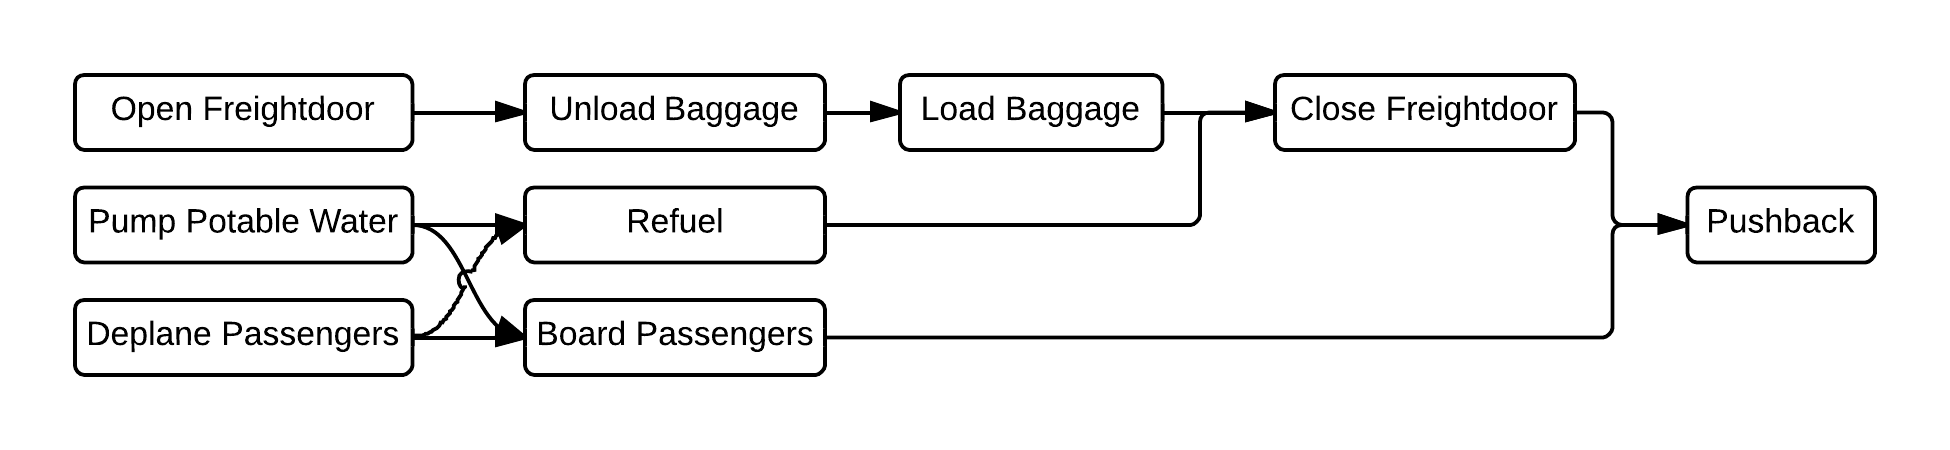
\includegraphics[width=230px]{Grafik/TestCase2Illu}
        \caption{\footnotesize An example of a flight graph}
    \end{figure}
\end{frame}

\subsection{Models}
\subsubsection{Classes}
\begin{frame}{Classes}{}
    \begin{figure}[H]
        \centering
        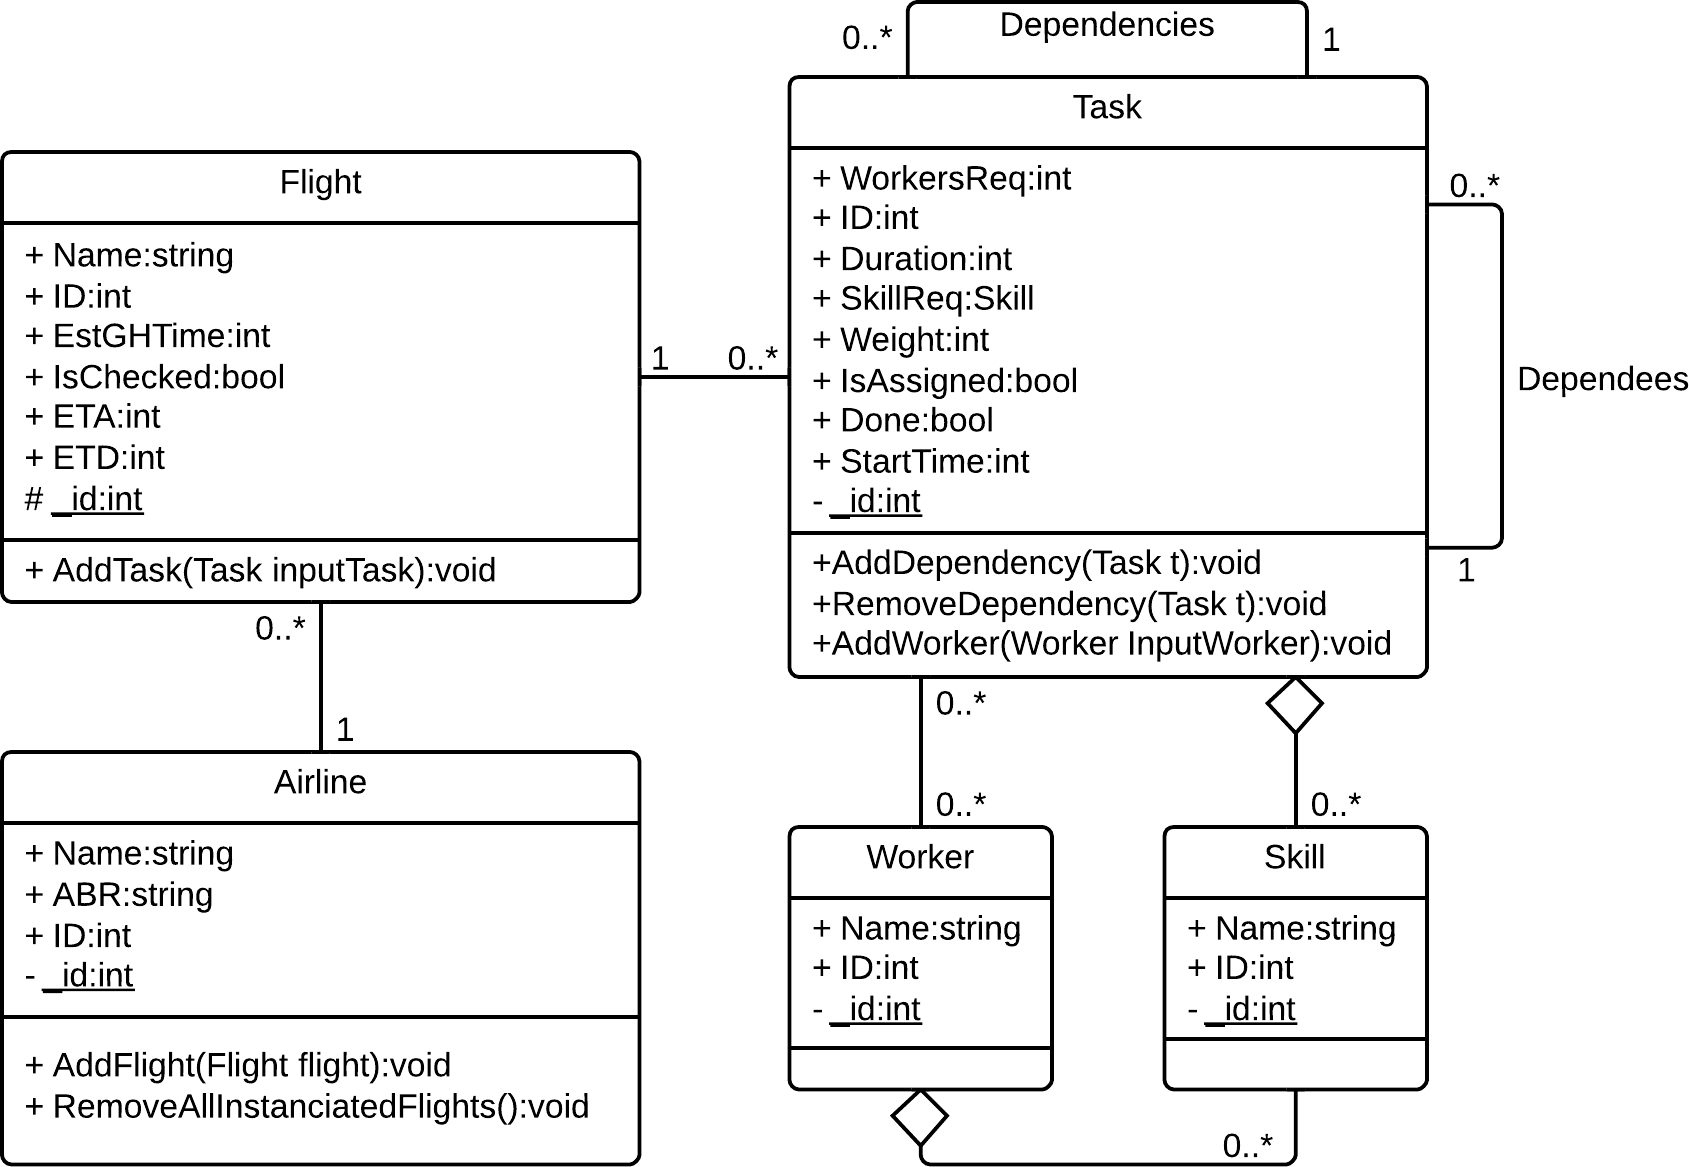
\includegraphics[width=230px]{Grafik/UML}
        \caption{\footnotesize UML of classes}
    \end{figure}
\end{frame}

\subsection{Views}
\subsubsection{MainWindow}
\begin{frame}{MainWindow}{}
    \begin{figure}[H]
        \centering
        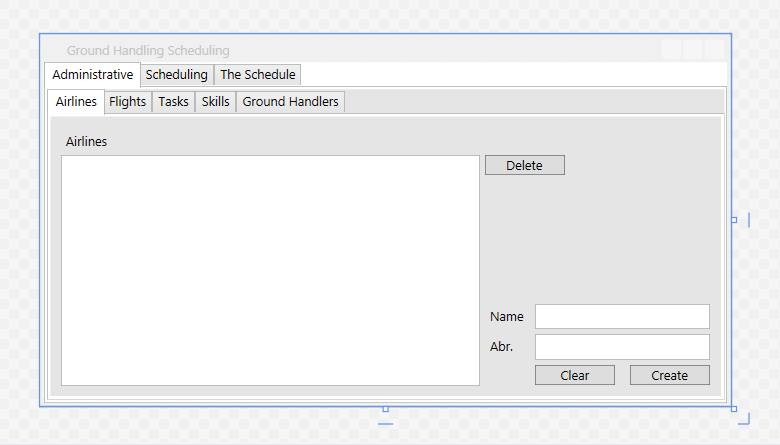
\includegraphics[width=230px]{Grafik/mainwindow}
        \caption{\footnotesize Main window of the program}
    \end{figure}
\end{frame}

\subsubsection{TimeAsker}
\begin{frame}{TimeAsker}{}
    \begin{figure}[H]
        \centering
        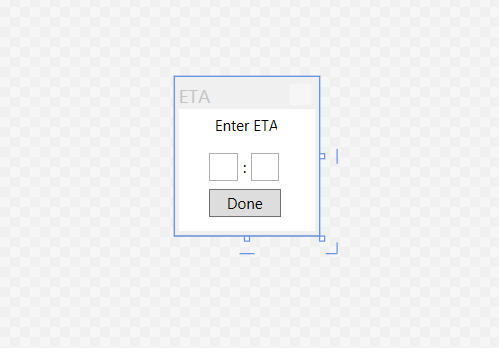
\includegraphics[width=230px]{Grafik/timeasker}
        \caption{\footnotesize ETA query for airplanes}
    \end{figure}
\end{frame}

\subsubsection{ListHandler}
\begin{frame}{ListHandler}{}
    \begin{figure}[H]
        \centering
        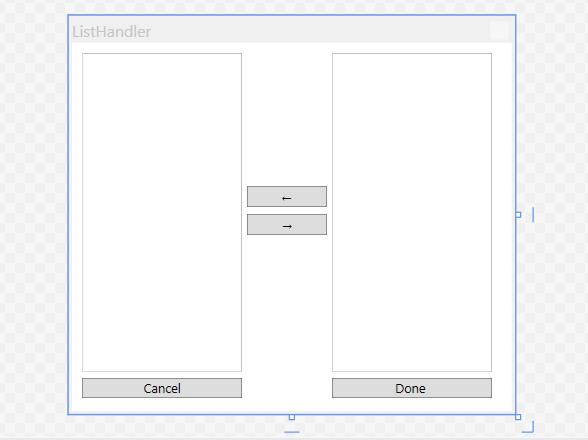
\includegraphics[width=230px]{Grafik/listhandler}
        \caption{\footnotesize Window for handling list-based selections}
    \end{figure}
\end{frame}

\subsection{Controllers}
\subsubsection{Schedule}
\begin{frame}[fragile]
\frametitle{Schedule}
\fontsize{8pt}{7}\selectfont
\begin{lstlisting}{style=cSharp}
pendingTasks.Sort((a, b) => b.Weight.CompareTo(a.Weight));
int i = 0;
while(i < pendingTasks.Count()) {
  if(assignWorker(pendingTasks[i],
      workForce.Values.ToList(), currentTime)) {
    addEvent(pendingTasks[i], currentTime +
      pendingTasks[i].Duration, eventList);
    pendingTasks.Remove(pendingTasks[i]);
  } else {
    i++;
  }
}
\end{lstlisting}
\end{frame}

\newpage

\subsubsection{CalcWeight}
\begin{frame}[fragile]
\frametitle{CalcWeight}
\fontsize{8pt}{7}\selectfont
\begin{lstlisting}{style=cSharp}
public static void CalcWeight(TaskInstance curN, int weight) {
  if((curN.Duration * curN.WorkersReq) + weight > curN.Weight)
    curN.Weight = (curN.Duration * curN.WorkersReq) + weight;
  if(curN.Dependencies.Count != 0) {
    foreach(TaskInstance Nd in curN.Dependencies)
      CalcWeight(Nd, curN.Weight);
  }
}
\end{lstlisting}
\end{frame}

\newpage

\subsubsection{AssignWorker}
\begin{frame}[fragile]
\frametitle{AssignWorker}
\fontsize{8pt}{7}\selectfont
\begin{lstlisting}{style=customc}
public static bool AssignWorker(TaskInstance inputTask,
    List<Team> workForce, int currentTime) {
  List<Team> PossibleWorkers = new List<Team>();
  PossibleWorkers.AddRange(workForce.Where(
    t => t.Skills.Exists(
    x => x.Name == inputTask.SkillReq.Name)));
  PossibleWorkers = PossibleWorkers.Where(
    x => checkTaskConflicts(inputTask, x.Tasks,
    currentTime)).ToList();
  PossibleWorkers.Sort(
    (x, y) => x.Skills.Count.CompareTo(y.Skills.Count));
  if(PossibleWorkers.Count() >= inputTask.WorkersReq) {
    for(int i = 0; i < inputTask.WorkersReq; i++) {
      inputTask.StartTime = currentTime;
      inputTask.AddWorker(PossibleWorkers[i]);
    }
    inputTask.IsAssigned = true;
    return true;
  } else {
  return false;
  }
}
\end{lstlisting}
\end{frame}

\newpage

\subsubsection{CheckForLoop}
\begin{frame}[fragile]
\frametitle{CheckForLoop}
\fontsize{8pt}{7}\selectfont
\begin{lstlisting}{style=customc}
public bool CheckForLoop(Task inputTask, Task checkTask) {
  foreach(Task t in inputTask.Dependencies) {
    if(t == checkTask) {
      return true;
    } else {
      return CheckForLoop(t, checkTask);
    }
  }
  return false;
}
\end{lstlisting}
\end{frame}